%%%%%%%%%%%%%%%%%%%%%%%%%%%%%%%%%%%%%%%%%%%%%%%%%%%%%%%%%%%%%%%%%%
\section{Verification benchmark suite}\label{sec:benchmark_suite}
%%%%%%%%%%%%%%%%%%%%%%%%%%%%%%%%%%%%%%%%%%%%%%%%%%%%%%%%%%%%%%%%%%
% Every number in this section is traceable to paper-data/benchmark_inventory.md
% / benchmarks.yaml, which cite the solids4foam development-branch
% verification READMEs, reference JSON/CSV files and PR descriptions
% (inventory commit 7c928c55; no FSI tutorial changes up to c706be68).
% Values marked (derived) in comments were computed in the inventory from
% tabulated values; values marked (read from plot) are approximate.

The benchmarks are grouped by the quality of their reference (Table~\ref{tab:ref_hierarchy}) rather than by geometry or regime: problems with exact references (Section~\ref{sec:exact_refs}), problems with independently converged numerical references (Section~\ref{sec:independent_refs}), classical benchmarks whose published values are re-examined (Section~\ref{sec:classical}), three-dimensional problems of increasing geometric complexity (Section~\ref{sec:threeD}), and an additional transient problem (Section~\ref{sec:additional}).
Table~\ref{tab:suite_overview} summarises the suite and the verification evidence currently available for each case.
All calculations use the cell-centred finite volume fluid and solid solvers of solids4foam~\citep{Cardiff2025} with partitioned coupling; the second-order \texttt{backward} (BDF2) time scheme is used unless stated.

\begin{table}[htbp]
	\centering
	\footnotesize
	\setlength{\tabcolsep}{3pt}
	\caption{Overview of the benchmark suite and of the verification evidence currently available. Ref.: reference category (Table~\ref{tab:ref_hierarchy}). Mesh and $\Delta t$: number of levels in the refinement study (``scaled'' denotes $\Delta t$ reduced with $h$ in the mesh study, with no separate time study). Coupling: comparison of two coupling algorithms (IQN-ILS, Robin--Neumann (RN) or Aitken), or a coupling-tolerance sweep.}
	\label{tab:suite_overview}
	\begin{tabular}{llllllll}
		\toprule
		Case & Dim. & Regime & Solid & Ref. & Mesh & $\Delta t$ & Coupling \\
		\midrule
		ringAddedMass & 2-D & free vibration & small & A & 3 & 3 & IQN-ILS/RN \\
		womersleyTube & axisym. & periodic (forced) & small & A & 3 & 3 & IQN-ILS/RN \\
		collapsibleChannel & 2-D & transient & large & B & 4 (fluid) & 4 & IQN-ILS/RN; $\rho_s$ sweep \\
		Hron--Turek FSI1 & 2-D & steady & large & B & 2 & 2 & IQN-ILS/RN \\
		Hron--Turek FSI3 & 2-D & self-excited & large & C & 2 & scaled & IQN-ILS/RN \\
		Hron--Turek FSI2 & 2-D & self-excited & large & C & 2 & scaled & tolerance sweep \\
		3dTube & 3-D & transient pulse & small & C-weak & 2 & 4 & IQN-ILS/RN \\
		mokLidDrivenCavity & 2-D & periodic (forced) & large & C-weak & 4 & 3 & IQN-ILS/Aitken$^\dagger$ \\
		cavityFlexibleBottom$^\ast$ & 2-D & steady & large & C-weak & 3 & -- & none \\
		beamInCrossFlow$^\ast$ & 3-D & steady & small/large & C/C-weak & 4/5 & scaled & IQN-ILS/RN \\
		Hessenthaler$^\ast$ & 3-D & periodic & large & -- & -- & -- & -- \\
		blobInTreacle$^\ast$ & 2-D & trans.\,$\to$\,steady & large & C-weak & 4 & 4 & none \\
		\bottomrule
		\multicolumn{8}{l}{$^\ast$ Provisional (Sections~\ref{sec:cavity}, \ref{sec:beam}, \ref{sec:hessenthaler}, \ref{sec:blob}). $^\dagger$ Iteration counts only; no quantitative difference recorded.}
	\end{tabular}
\end{table}

\todo{Insert a figure panel with geometry sketches for ringAddedMass, womersleyTube, collapsibleChannel and mokLidDrivenCavity; geometry figures currently exist only for HronTurek, 3dTube, beamInCrossFlow, cavityFlexibleBottom and blobInTreacle (figures/*-geometry.pdf).}


%%%%%%%%%%%%%%%%%%%%%%%%%%%%%%%%%%%%%%%%%%%%%%%%%%%%%%%%%%%%%%%%%%
\subsection{Exact and semi-analytical reference problems}\label{sec:exact_refs}
%%%%%%%%%%%%%%%%%%%%%%%%%%%%%%%%%%%%%%%%%%%%%%%%%%%%%%%%%%%%%%%%%%

Both problems in this group are linear, small-amplitude problems whose exact solution is obtained from the continuum equations by a one-dimensional spectral (Chebyshev collocation) calculation that converges to near round-off.
They are therefore category A, and the total error of the coupled calculation can be measured directly, not inferred from self-convergence.
The collocation scripts are stored with the cases and are independent of solids4foam, although they were written by the same authors.

%%-------------------------------------------------------------------
\subsubsection{Ring added-mass problem}\label{sec:ring}
%%-------------------------------------------------------------------

\paragraph{Purpose.}
Added mass is the principal source of instability and slow convergence in partitioned FSI~\citep{Causin2005}.
Most benchmarks contain an added-mass effect of fixed, unquantified strength.
This problem isolates it: the fluid lowers the natural frequency of an elastic ring by an amount that linear theory gives exactly, and the strength of the effect is varied over two decades at fixed solid properties.

\paragraph{Problem.}
An elastic ring vibrates freely in its $n=2$ (ovalling) mode inside a fluid-filled rigid annulus (plane strain; a quarter of the domain is modelled with symmetry conditions).
The fluid is incompressible with $\nu_f = 10^{-7}\,\mathrm{m^2/s}$, i.e.\ effectively inviscid; the Stokes layer is deliberately not resolved.
The amplitude is approximately $5\times10^{-4}$ of the ring radius and the solid is modelled with linear geometry.
Three fluid densities give mass ratios $\mu = 0.101$, $1.008$ and $10.08$ (``weak'', ``moderate'', ``strong''), and a dry (in vacuo) run is made on each mesh.
\todo{Add a short parameter table (ring radii, thickness, $E$, $\nu$, $\rho_s$, outer wall radius) from the tutorial README, and the definition of $\mu$.}

\paragraph{Reference.}
The reference (category A) is the exact linear eigenvalue of a plane-strain continuum ring loaded by the exact potential-flow added-mass traction, computed by Chebyshev collocation with 24 intervals; refining the collocation changes the frequencies by approximately $5\times10^{-8}$.
The classical thin-ring frequency with the confined added mass of Brennen~\citetodo{Brennen 1982, NCEL report CR 82.010; not in bibliography} agrees with it to $O((h/a)^2)$ and serves as a check.
The exact dry frequency is $\omega_\mathrm{dry} = 2.555042\,\mathrm{rad/s}$, and the wet frequencies are $2.435615$, $1.804513$ and $0.768654\,\mathrm{rad/s}$ for the three levels.
A linearised viscous solution, also stored, shifts these by $-0.004\%$, $-0.026\%$ and $-0.073\%$, which bounds the effect of the small fluid viscosity.

\paragraph{Verification study.}
Frequencies are measured from zero crossings over four periods.
The mesh study uses refinement factors 1, 2 and 4 (solid $4\times48$ to $16\times192$ cells; fluid $12\times48$ to $48\times192$) at 100 steps per period, and the time-step study uses 25, 50 and 100 steps per period on the middle mesh.
Two solid discretisations are compared (the standard second-order residual and a cubic high-order residual), as are the IQN-ILS and Robin--Neumann couplings.
Table~\ref{tab:ring} gives representative results.

\begin{table}[htbp]
	\centering
	\small
	\setlength{\tabcolsep}{5pt}
	\caption{ringAddedMass: frequency error against the exact continuum solution and error of the wet/dry frequency ratio (high-order solid, IQN-ILS). Mesh: refinement factor; steps: time steps per period. Source: solids4foam \texttt{ringAddedMass/verification/README.md}.}
	\label{tab:ring}
	\begin{tabular}{lrrrrr}
		\toprule
		Level & Mesh & Steps & $\omega$ (rad/s) & Error in $\omega$ & Error in ratio \\
		\midrule
		dry & 1 & 100 & 2.55254 & $-0.098\%$ & -- \\
		dry & 4 & 100 & 2.55173 & $-0.129\%$ & -- \\
		dry & 2 & 25 & 2.50576 & $-1.929\%$ & -- \\
		strong ($\mu=10.08$) & 1 & 100 & 0.76843 & $-0.029\%$ & $+0.068\%$ \\
		strong & 2 & 100 & 0.76796 & $-0.090\%$ & $+0.021\%$ \\
		strong & 4 & 100 & 0.76770 & $-0.124\%$ & $+0.006\%$ \\
		strong & 2 & 25 & 0.75477 & $-1.806\%$ & $+0.125\%$ \\
		strong & 2 & 50 & 0.76552 & $-0.408\%$ & $+0.087\%$ \\
		\bottomrule
	\end{tabular}
\end{table}

\paragraph{Findings.}
\begin{itemize}
	\item \emph{Time.} The observed temporal orders of the frequency are 1.90, 1.92, 2.02 and 2.14 (dry, weak, moderate, strong), consistent with BDF2. Richardson extrapolation in time brings every frequency to within $+0.018\%$ of the exact value. The residual error of approximately $-0.13\%$ at 100 steps per period is therefore the phase error of the time scheme, not a coupling or spatial error.
	\item \emph{Space.} With the high-order solid the frequencies change by at most $0.06\%$ between meshes, too little to define a spatial order: the frequency is spatially converged on the coarsest mesh, and the slight growth of $|\text{error}|$ with refinement in Table~\ref{tab:ring} reflects the removal of a small spatial error that partly offsets the temporal one. The wet/dry ratio, in which the common time error cancels, converges at observed orders 1.77, 1.73 and 1.68 to $+0.001\%$, $+0.003\%$ and $+0.006\%$ on the finest mesh.
	\item \emph{Solid discretisation.} The standard second-order solid is $20.7\%$ too stiff in bending on the coarsest mesh and $1.6\%$ on the finest (observed order 1.66), whereas the high-order solid is within $0.13\%$ on every mesh. Nevertheless the wet/dry ratio of the two solids agrees to $0.003\%$ on the finest mesh: the added-mass coupling is verified independently of the accuracy of the solid discretisation.
	\item \emph{Coupling.} IQN-ILS and Robin--Neumann agree to $0.03\%$ in frequency. Mean coupling iterations per step are 2.99, 3.95 and 4.91 for IQN-ILS and 3.87, 4.85 and 12.29 for Robin--Neumann (weak to strong).
	\item \emph{Unresolved.} The IQN-ILS solutions lose amplitude at a rate that depends on the mesh and the added mass (up to $2.1\%$ per period on the coarsest mesh at the strong level, halving with each refinement), whereas the Robin--Neumann solutions are almost undamped ($\leq0.05\%$ per period on the middle mesh). The mechanism has not been identified. It does not affect the frequency at the reported precision.
\end{itemize}

\paragraph{Role in the suite.}
This is the only case with an exact reference and a controlled added-mass ratio spanning two decades.
Because dry and wet runs share the solid and time discretisations, the wet/dry ratio isolates the fluid--solid coupling from the solid and temporal errors.
The problem is inexpensive (the full study of 35 runs takes about 30\,min on 32 cores; the tutorial about 75\,s serial).
Its limitations are that viscous effects are, by design, not verified, and that only small-amplitude linear dynamics are tested.

%%-------------------------------------------------------------------
\subsubsection{Pulsatile compliant tube}\label{sec:womersley}
%%-------------------------------------------------------------------

\paragraph{Purpose.}
Pressure-wave propagation in a compliant vessel combines added mass, viscous attenuation and wall compliance, and is the canonical haemodynamic FSI configuration.
Womersley's analysis~\citetodo{Womersley 1955 Phil.\ Mag.; Womersley 1957 Phys.\ Med.\ Biol.} has been used to verify FSI codes before~\citetodo{Filonova et al.\ 2020, IJNMBE e3266}, usually in a thin-wall, long-wave form whose own modelling error is not negligible for a thick wall.

\paragraph{Problem.}
A harmonic pressure wave travels along an axisymmetric elastic tube (modelled as a $1^\circ$ wedge) of inner radius $R = 1\,\mathrm{m}$, wall thickness $h/R = 0.1$ and length $L = 15\,\mathrm{m}$, at Womersley number $\alpha = 5.01$ and mass ratio $\rho_s h/(\rho_f R) = 0.1$.
The wall is free to move axially (untethered).
The finite segment reproduces the infinite-tube solution because the exact travelling-wave data are imposed at both ends, so no reflection is generated, and the fields are initialised with the exact solution.
The wall radial displacement is approximately $5\times10^{-4}R$ and the peak velocity approximately $1.5\times10^{-3}$ of the wave speed, so the linear theory is appropriate and differences much below $10^{-3}$ are not expected to be meaningful.

\paragraph{Reference.}
The reference (category A) is the exact linear solution of the continuum problem: a thick linear-elastic cylinder (Chebyshev collocation, 16 intervals) coupled to the full linearised Navier--Stokes equations, with the complex wave number found from the frequency equation.
Collocation with 8 and 24 intervals agrees to approximately $10^{-11}$.
The solution reduces to Womersley's thin-wall equation, in the form of Filonova et al.\ (their Eq.~41), as $h/R\to0$, and agrees with the tethered long-wave limit to $2\times10^{-5}$.
The exact wave number is $k = 0.143978 - 0.020727\mathrm{i}\,\mathrm{m^{-1}}$, i.e.\ a wave speed of $0.872796\,\mathrm{m/s}$.
Womersley's thin-wall wave speed is $4.7\%$ higher for this wall thickness; using it as the reference would have hidden discretisation errors of the size studied here.

\paragraph{Verification study.}
The QoIs are the first Fourier coefficients at the forcing frequency, over the fifth and sixth periods, of: the axial velocity profile at $x = L/2$ (maximum error over the radius), the flow rate (amplitude and phase), the wall radial displacement at $L/2$ (amplitude and phase), and the wave speed and attenuation fitted to the pressure along the tube.
The mesh study refines all directions by factors 1, 2 and 4 (from 32 axial, 10 fluid-radial and 4 wall-radial cells) at 200 steps per period; the time-step study uses 50, 100 and 200 steps per period on the middle mesh; both use Robin--Neumann coupling.
IQN-ILS and Robin--Neumann are compared at 100 steps per period.
The change of the wall-displacement coefficient between the fifth and sixth periods is below $10^{-4}$ in every run.

\begin{table}[htbp]
	\centering
	\small
	\setlength{\tabcolsep}{5pt}
	\caption{womersleyTube: observed orders from successive differences (three levels) and finest-mesh errors against the exact solution (mesh factor 4, 200 steps per period). The profile mesh order is from its errors on the two finest meshes. Phases in radians. Source: solids4foam \texttt{womersleyTube/verification/README.md}.}
	\label{tab:womersley}
	\begin{tabular}{lrrr}
		\toprule
		Quantity & Mesh order & Time order & Finest-mesh error \\
		\midrule
		velocity profile (max.) & 2.06 & -- & $1.18\times10^{-3}$ \\
		flow-rate amplitude & 2.16 & 1.64 & $-7.15\times10^{-4}$ \\
		flow-rate phase & 1.92 & 1.84 & $1.5\times10^{-5}$ \\
		wall displacement amplitude & 2.15 & 1.71 & $8.57\times10^{-4}$ \\
		wall displacement phase & 0.97 & 1.74 & $-1.88\times10^{-3}$ \\
		wave speed & 2.48 & 1.29 & $8.93\times10^{-4}$ \\
		attenuation, $\mathrm{Im}(k)$ & 0.63 & 1.51 & $-4.47\times10^{-3}$ \\
		\bottomrule
	\end{tabular}
\end{table}

\paragraph{Findings.}
\begin{itemize}
	\item \emph{Space.} The velocity profile, flow rate, wall-displacement amplitude and wave speed converge at approximately second order in space (Table~\ref{tab:womersley}), and on the finest mesh agree with the exact solution to $0.12\%$ or better. The wall-displacement phase and the attenuation converge at only about first order, and the attenuation has the largest error, $-0.45\%$. Since $\mathrm{Im}(k)$ is only $14\%$ of $\mathrm{Re}(k)$, a given error in the fitted wave number is about seven times larger relative to the attenuation; the reason for the first-order phase convergence has not been established.
	\item \emph{Time.} The observed temporal orders are 1.29--1.84, \emph{below} the nominal second order of the BDF2 scheme that is used in both the fluid and the solid and in the interface-velocity condition. The cause has not been identified. Because the reference is exact, this finding is not an artefact of an imperfect reference: it is a property of the coupled discretisation (or of the start-up, see below) that a benchmark with a weaker reference could not have exposed.
	\item \emph{Start-up.} A transient of approximately $0.5\%$ in the wall displacement remains over the first period even though the fields are initialised exactly, and it \emph{grows} as the time step is reduced. One candidate is an inconsistency between the exact initial point displacements used to move the fluid mesh and the solid model's interpolation of its cell values. A start-up correction made elsewhere in the code for a different time scheme has been checked and does not apply to the \texttt{backward} scheme used here. Six periods are run and the last two are analysed to avoid contamination by this transient.
	\item \emph{Space--time interaction.} At 200 steps per period the temporal error is of the same size as the spatial error on the finest mesh. The successive-difference mesh orders cancel this common error, but the finest-mesh errors in Table~\ref{tab:womersley} contain it.
	\item \emph{Coupling.} IQN-ILS and Robin--Neumann agree to $3\times10^{-4}$ or better in every QoI (14.8 and 8.7 coupling iterations per step, respectively).
\end{itemize}

\todo{Do NOT remove or soften the sub-nominal temporal order. Planned diagnosis (paper-data/manuscript\_todos.md): time study on mesh factor 4 and at 400 steps per period; isolate the interface-velocity condition and the start-up transient. If the cause is found, report both the diagnosis and the corrected order; if not, retain the present statement as an open finding. Also note: the Robin--Neumann result moved by $0.26\%$ of amplitude between OpenFOAM-v2412 and v2512 (PR \#513 comment), which is larger than several of the finest-mesh errors in Table~\ref{tab:womersley} and must be resolved before the final numbers are fixed.}

\paragraph{Role in the suite.}
This is the only viscous, time-periodic, wave-propagation case with an exact reference, and the only axisymmetric case.
It complements ringAddedMass (inviscid, standing mode) and provides separate amplitude and phase QoIs.
Its central result for this paper is a negative one: an exact reference exposes a sub-nominal temporal order and a slow, first-order convergence of phase and attenuation that are not visible in the more widely used benchmarks.
Limitations: the tube wall is untethered, unlike Womersley's constrained tube, because a suitable mixed displacement--traction condition is not yet available for the solid solver used (solids4foam issue \#511); the high-order solid residual cannot be used on wedge meshes (issue \#512); the evidence was recorded on one OpenFOAM version and platform.


%%%%%%%%%%%%%%%%%%%%%%%%%%%%%%%%%%%%%%%%%%%%%%%%%%%%%%%%%%%%%%%%%%
\subsection{Independently resolved numerical benchmarks}\label{sec:independent_refs}
%%%%%%%%%%%%%%%%%%%%%%%%%%%%%%%%%%%%%%%%%%%%%%%%%%%%%%%%%%%%%%%%%%

The two problems in this group have no analytical solution, but have references computed with independent codes, discretisations and solution strategies, each with its own convergence evidence (category B).
Differences between the present results and the reference are interpreted only where they exceed the reference uncertainty.

%%-------------------------------------------------------------------
\subsubsection{Collapsible channel}\label{sec:collapsible}
%%-------------------------------------------------------------------

\paragraph{Purpose.}
A thin, very light elastic wall in a channel carrying internal flow combines strong added mass, bending-dominated large deformation and fluid-mesh motion.
Flow in collapsible channels is a classical FSI problem~\citetodo{Jensen \& Heil 2003, J.\ Fluid Mech.}~\citep{Heil2004, Heil2008}, and the strongly coupled internal-flow configuration is precisely where partitioned methods are least robust.

\paragraph{Problem.}
A two-dimensional channel with an elastic section of its upper wall (thickness $h/L = 0.005$) is subjected to a ramped external pressure; the wall collapses to approximately $21\%$ of the channel width at the first trough and then performs a damped oscillation of period approximately $0.8\,\mathrm{s}$, analysed to $t = 1.5\,\mathrm{s}$.
The flow has $Re = Re\,St = 50$ and is driven by an imposed pressure drop with Poiseuille inflow.
The solid is a total-Lagrangian St Venant--Kirchhoff continuum.
A small regularising wall density $\rho_s = \rho_f$ is used.

The problem is a \emph{modified} version of the published configuration of Jensen and Heil: the wall has no pre-stress ($\sigma_0 = 0$), $h/a = 1/20$, clamped ends, a pressure ramp and the regularising density.
The regularising density shifts the response by $0.28\%$ of the peak displacement relative to a massless wall.
These modifications are made so that the problem is well posed for a continuum solid and for partitioned coupling; the results therefore verify the code on this modified problem and do not reproduce the published values.

\paragraph{Reference and controlled model-form difference.}
The reference (category B) is computed with oomph-lib\citetodo{Heil \& Hazel 2006, oomph-lib}, a monolithic Newton finite element code, with Taylor--Hood (Q2Q1) or Crouzeix--Raviart (Q2P-1) fluid elements and a geometrically nonlinear Kirchhoff--Love \emph{beam} for the wall, using BDF2 for the fluid and a Newmark scheme for the beam.
The driver source is stored with the case, so the reference can be regenerated.
The converged reference is a Richardson extrapolation in time from $\Delta t = 0.003125$ and $0.0015625\,\mathrm{s}$; its uncertainty is approximately $0.3\%$ of the peak displacement, dominated by the oomph-lib spatial error (refinement levels 1 and 2 differ by $0.26\%$; the Richardson correction is $0.06\%$; the two fluid element types differ by less than $0.001\%$).

The comparison contains a deliberate, controlled \emph{model-form} difference: oomph-lib represents the wall as a geometrically nonlinear beam, whereas solids4foam resolves it as a two-dimensional continuum.
The difference is of order $h/L$; for the static deflection under the steady load it is $0.05\%$, which is used as an estimate of the model-form contribution.
A difference between the two solutions below approximately $0.3\%$ of the peak (reference uncertainty) plus this model-form contribution cannot be attributed to either code.

\paragraph{Verification study.}
The QoI is the vertical displacement history of the wall midpoint (and quarter points), with the first trough as a scalar summary.
Four studies are performed: a static wall test; a solid-discretisation comparison (cubic high-order versus linear least-squares reconstruction); a fluid-mesh study (four levels, 3\,200 to 51\,200 fluid cells, Robin--Neumann coupling, fixed $\Delta t = 0.00625\,\mathrm{s}$, compared with oomph-lib at the same $\Delta t$); and a time-step study ($\Delta t = 0.025$ to $0.003125\,\mathrm{s}$ on the coarsest fluid mesh).
The coupling study compares IQN-ILS and Robin--Neumann and maps the range of wall densities for which each completes, from $\rho_s/\rho_f = 0$ to 3.

\begin{figure}[htbp]
	\centering
	% Source: solids4foam development, tutorials/fluidSolidInteraction/collapsibleChannel/verification/reference/mesh_study_wallMid.png (PR #507).
	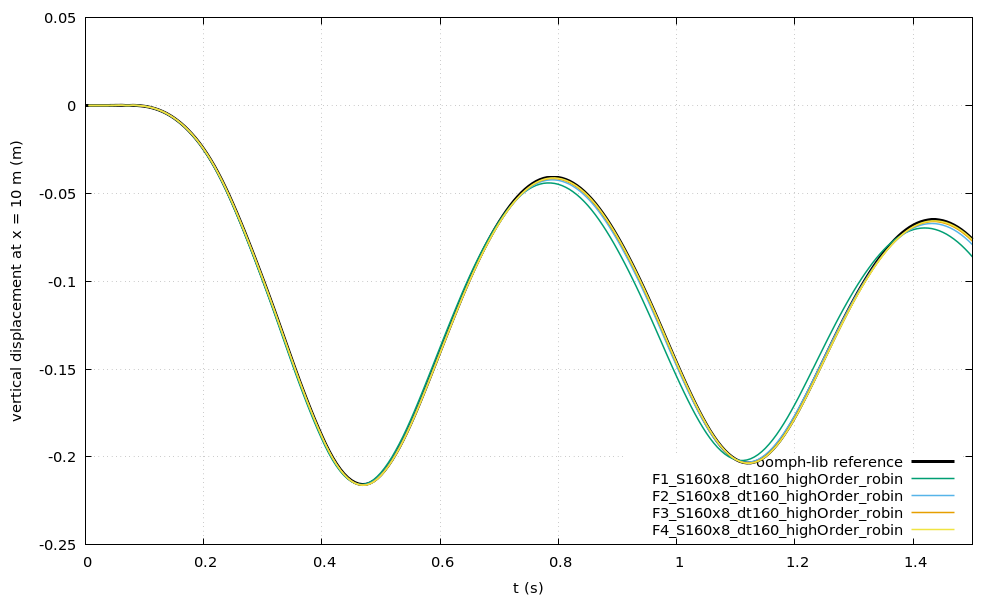
\includegraphics[width=0.85\textwidth]{figures/verification/collapsibleChannel_mesh_study_wallMid}
	\caption{collapsibleChannel: wall-midpoint vertical displacement for fluid-mesh levels F1--F4 (solid mesh $160\times8$, $\Delta t = 0.00625\,\mathrm{s}$, high-order solid, Robin--Neumann coupling) against the oomph-lib reference. Interim figure reproduced from the solids4foam verification output.}
	\label{fig:collapsible_mesh}
\end{figure}
\todo{Replace Figure~\ref{fig:collapsible_mesh} with a publication-quality version (legend labels, inset at first trough and second peak, error-versus-$h$ panel). The current PNG legend shows raw run identifiers.}

\paragraph{Findings.}
\begin{itemize}
	\item \emph{Static wall.} The cubic solid is within $0.25\%$ of the oomph-lib static deflection on all solid meshes and converges to a $0.05\%$ difference, the beam--continuum model-form difference. The linear-reconstruction solid has errors from $-16.7\%$ to $-0.22\%$ (approximately second order in the in-plane spacing).
	\item \emph{Solid in the coupled problem.} On the tutorial mesh the cubic solid contributes $0.44\%$ error, against $17.4\%$ for the linear reconstruction. For a thin bending-dominated wall the solid discretisation can thus dominate the FSI error unless a high-order or well-resolved solid is used.
	\item \emph{Fluid mesh.} The error against oomph-lib at the same $\Delta t$ falls from $4.65\%$ to $1.43\%$, $0.53\%$ and $0.50\%$ of the peak displacement (observed orders 1.7 and 2.4, then a floor) (Fig.~\ref{fig:collapsible_mesh}). The floor coincides with the reference uncertainty of approximately $0.3\%$ plus the model-form contribution; the finest-mesh first trough is $-0.21610\,\mathrm{m}$ against $-0.2160\,\mathrm{m}$ for the converged oomph-lib reference.
	\item \emph{Time step.} Successive differences of $4.56\%$, $1.33\%$ and $0.34\%$ give orders 1.8 and 2.0; oomph-lib itself shows 1.8 and 1.9 on the same sequence.
	\item \emph{Coupling.} IQN-ILS and Robin--Neumann agree to $0.08$--$0.23\%$ of the peak, but this gap does \emph{not} decrease with mesh refinement; it is of the size expected from the coupling tolerance and is therefore an iterative, not a discretisation, error. In the density sweep IQN-ILS fails to complete for part of the range, whereas Robin--Neumann completes for all $\rho_s/\rho_f \geq 1$.
\end{itemize}

\paragraph{Role in the suite.}
This is the strongest independent-code comparison in the suite: a regenerable monolithic finite element reference, with its own time-convergence and spatial-uncertainty estimate, for a large-deformation, strongly added-mass internal flow.
It also shows that once the discretisation error falls to approximately $0.5\%$, the reference uncertainty, the model-form difference and the coupling tolerance are all of comparable size, so that further agreement cannot be expected without tightening all three.
Limitations: the temporal error on the finer fluid meshes has not been measured separately; the mesh and time studies follow separate refinement paths; the high-order solid is serial only, and a 4-rank run with the linear-reconstruction solid gave an incorrect displacement that remains to be re-checked.

%%-------------------------------------------------------------------
\subsubsection{Hron--Turek FSI1}\label{sec:fsi1}
%%-------------------------------------------------------------------

\paragraph{Purpose.}
FSI1 is the steady, low-Reynolds-number member of the Turek--Hron family~\citep{Turek2006}: an elastic flag attached to a rigid cylinder in a channel at $Re = 20$.
It tests steady coupling with small loads and small (but geometrically nonlinear) deformation, and it has the best-converged published reference of the classical benchmarks.

\paragraph{Reference.}
The Featflow results for FSI1 are tabulated on six mesh levels (2+0 to 7+0, the finest with approximately $10^6$ elements); the spread across these levels is $0.73\%$ in $u_x$, $0.19\%$ in $u_y$, $0.14\%$ in drag and $0.26\%$ in lift.
The finest values ($u_x = 2.2705\times10^{-5}\,\mathrm{m}$, $u_y = 8.2088\times10^{-4}\,\mathrm{m}$, drag $14.2943\,\mathrm{N/m}$, lift $0.76375\,\mathrm{N/m}$) are therefore treated as an independently converged (category-B) reference.
\todo{Cite the Featflow table source precisely (Turek--Hron benchmark web pages / Turek et al.\ 2010 book chapter?)~\citetodo{Featflow FSI benchmark tables}; confirm that the six-level spread quoted is from that source.}

\paragraph{Verification study.}
The steady state is reached by pseudo-transient integration to $t = 30\,\mathrm{s}$.
Two mesh levels (1x and 2x; the 4x level is defined but has not been run) are compared with the Featflow finest level, and two time steps ($\Delta t = 0.025$ and $0.01\,\mathrm{s}$) are compared on the 1x mesh.
Steady IQN-ILS and Robin--Neumann solutions are compared, and the fluid solver tolerance is varied from $10^{-6}$ to $10^{-9}$.

\paragraph{Findings.}
On the 2x mesh the errors are $0.97\%$ in $u_x$, $4.64\%$ in $u_y$, $0.24\%$ in drag and $1.55\%$ in lift (1x: $u_y = 7.0426\times10^{-4}\,\mathrm{m}$; 2x: $7.8282\times10^{-4}\,\mathrm{m}$).
The two-level apparent orders against the Featflow finest level are 1.5--1.7.
The pseudo-time step changes $u_y$ and drag by $0.04\%$ and $u_x$ by $0.26\%$; the coupling algorithms agree to $0.01\%$; the fluid solver tolerance changes the steady values by at most $2\times10^{-4}$.
The transverse tip displacement $u_y$ is thus the slowest-converging QoI, even though the drag is already within $0.25\%$ on the 2x mesh.

\paragraph{Role in the suite.}
FSI1 is the cheapest category-B problem with large-deformation kinematics (1x: 781\,s serial; 2x: 3\,062\,s on 2 ranks) and is a natural first steady FSI check.
With only two levels, however, no reference-free order is available, and the apparent orders (1.5--1.7) are below the formal order; a third level is needed to establish whether the sequence is asymptotic.
\todo{Run the 4x level (estimated $>14$\,h on 3 ranks) to obtain a three-level, reference-free order for $u_y$. Without it, report FSI1 as ``converging towards the Featflow reference'' rather than ``verified to second order''.}


%%%%%%%%%%%%%%%%%%%%%%%%%%%%%%%%%%%%%%%%%%%%%%%%%%%%%%%%%%%%%%%%%%
\subsection{Classical FSI benchmarks revisited}\label{sec:classical}
%%%%%%%%%%%%%%%%%%%%%%%%%%%%%%%%%%%%%%%%%%%%%%%%%%%%%%%%%%%%%%%%%%

The benchmarks in this group are widely used, but their published values carry incompletely quantified error, are inconsistent between sources, or both.
For each, the present calculations are first established by self-convergence, and the comparison with the literature is then used to examine the published values themselves.

%%-------------------------------------------------------------------
\subsubsection{Hron--Turek FSI2 and FSI3}\label{sec:fsi23}
%%-------------------------------------------------------------------

\begin{figure}[htbp]
	\centering
	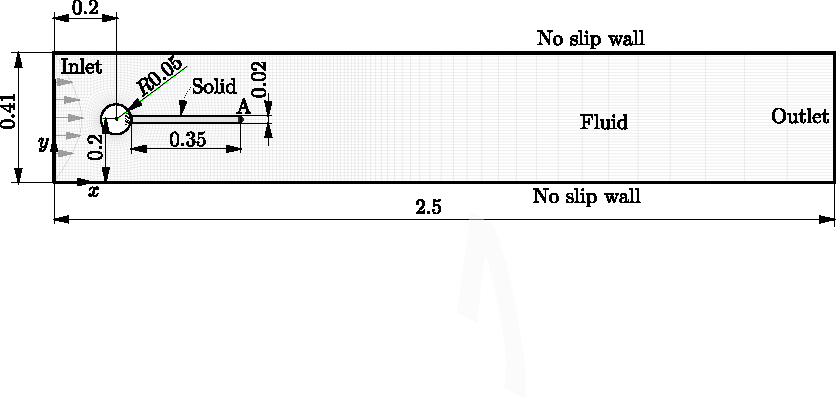
\includegraphics[scale=1]{figures/HronTurek3-geometry}
	\caption{Hron--Turek benchmark geometry (shown for FSI3; FSI1 and FSI2 share the geometry).}
	\label{fig:hronturek_geom}
\end{figure}

\paragraph{Purpose.}
FSI2 and FSI3 are the self-excited periodic members of the family~\citep{Turek2006} (Fig.~\ref{fig:hronturek_geom}).
FSI3 ($Re = 200$, $\rho_s = \rho_f$) tests a low mass ratio and a high-frequency vortex-induced oscillation of moderate amplitude ($u_y \approx \pm35\,\mathrm{mm}$); FSI2 ($Re = 100$, a heavier and softer flag) tests large-amplitude flapping ($u_y \approx \pm80\,\mathrm{mm}$) and the resulting distortion of the fluid mesh.

\paragraph{Reference and its ambiguity.}
The references are the Featflow level-4 tables (FSI3: $\Delta t = 0.00025\,\mathrm{s}$; FSI2: $\Delta t = 0.0005\,\mathrm{s}$).
For FSI2, the Featflow values change by $0.9$--$2.5\%$ between levels 3 and 4, so the reference itself is uncertain by approximately $1\%$; both cases are classed as category C.
The detailed Featflow tables differ from the summary values of~\citet{Turek2006} that are most often quoted (Table~\ref{tab:hronturek_ref}).
The largest difference is in the FSI3 drag amplitude ($22.66$ in the summary against $27.74\,\mathrm{N/m}$ in the table, $-18\%$); the summary frequencies are also rounded ($5.3$ against $5.46\,\mathrm{Hz}$ for FSI3 $u_y$; $2.0$ against $1.93\,\mathrm{Hz}$ for FSI2).
The present study uses the tables.
As a consistency check, the verification driver reproduces the tabulated statistics from the published Featflow time histories to within $0.7\%$ (FSI3; $1.1\%$ for the drag amplitude) and $0.3\%$ (FSI2).
A comparison with the summary values would misattribute an $18\%$ difference in FSI3 drag amplitude to the code under test.

\begin{table}[htbp]
	\centering
	\small
	\setlength{\tabcolsep}{5pt}
	\caption{Hron--Turek FSI3 and FSI2: frequently quoted summary values of~\citet{Turek2006} against the Featflow level-4 tables used here (amplitudes; frequencies in brackets). Units: mm for displacements, N/m for forces. Source: solids4foam \texttt{HronTurek/verification/README.md} and reference JSON.}
	\label{tab:hronturek_ref}
	\begin{tabular}{llll}
		\toprule
		Case & Quantity & Summary~\citep{Turek2006} & Featflow table \\
		\midrule
		FSI3 & $u_y$ amplitude & 34.38 [5.3\,Hz] & 34.99 [5.46\,Hz] \\
		FSI3 & drag amplitude & 22.66 & 27.74 \\
		FSI3 & lift amplitude & 149.78 & 153.91 \\
		FSI2 & $u_y$ amplitude & 80.6 [2.0\,Hz] & 81.6 [1.93\,Hz] \\
		FSI2 & drag amplitude & 73.75 & 77.65 \\
		FSI2 & lift amplitude & 234.2 & 237.8 \\
		\bottomrule
	\end{tabular}
\end{table}
\todo{Check every entry of Table~\ref{tab:hronturek_ref} against the original sources (2006 chapter and Featflow tables) rather than against the solids4foam README; identify which later papers quote which set.}

\paragraph{Verification study.}
Two mesh levels are run (1x: 5\,336 fluid and 630 solid cells; 2x: 21\,344 and 2\,520), with the time step halved with the mesh (FSI3: $\Delta t = 0.001$ and $0.0005\,\mathrm{s}$); a 4x level is defined but has not been run.
There is no separate time-step study.
The statistics are taken over the last full periods of the oscillation.
For FSI3, Robin--Neumann and IQN-ILS are compared from a common restart; for FSI2, the coupling tolerance (\texttt{outerCorrTolerance}) is swept over $10^{-5}$, $10^{-6}$ and $10^{-7}$.

\begin{table}[htbp]
	\centering
	\small
	\setlength{\tabcolsep}{5pt}
	\caption{Hron--Turek FSI3 and FSI2: relative errors against the Featflow tables on the 1x and 2x meshes (IQN-ILS), and two-level apparent order for FSI3. The 1x errors and the apparent orders were computed from the tabulated values in the evidence inventory.}
	\label{tab:hronturek}
	\begin{tabular}{lrrrrr}
		\toprule
		 & \multicolumn{3}{c}{FSI3} & \multicolumn{2}{c}{FSI2} \\
		\cmidrule(lr){2-4}\cmidrule(lr){5-6}
		Quantity & 1x & 2x & apparent order & 1x & 2x \\
		\midrule
		$u_x$ mean & $21.3\%$ & $3.1\%$ & 2.8 & $21.6\%$ & $3.1\%$ \\
		$u_x$ amplitude & $19.2\%$ & $2.1\%$ & 3.2 & $16.4\%$ & $1.9\%$ \\
		$u_y$ amplitude & $14.4\%$ & $2.3\%$ & 2.6 & $12.4\%$ & $1.3\%$ \\
		$u_y$ frequency & $2.5\%$ & $1.2\%$ & 1.1 & $6.9\%$ & $1.8\%$ \\
		drag mean & $0.7\%$ & $0.3\%$ & 1.5 & $4.6\%$ & $0.5\%$ \\
		drag amplitude & $15.5\%$ & $1.2\%$ & 3.8 & $13.1\%$ & $2.0\%$ \\
		lift amplitude & $48.9\%$ & $13.3\%$ & 1.9 & $7.9\%$ & $7.8\%$ \\
		\bottomrule
	\end{tabular}
\end{table}

\paragraph{Findings.}
\begin{itemize}
	\item \emph{Displacements and drag.} On the 2x mesh the displacement and drag statistics are within $1.2$--$3.1\%$ of the Featflow tables for both cases. The FSI3 two-level apparent orders (Table~\ref{tab:hronturek}) range from 1.1 to 3.8; such a spread, with values well above the formal order, indicates that the 1x mesh is outside the asymptotic range, and no order can be claimed from two levels.
	\item \emph{Lift amplitude.} The lift amplitude is the slowest-converging QoI. For FSI3 its error falls from $48.9\%$ to $13.3\%$; for FSI2 it is $7.9\%$ on 1x and $7.8\%$ on 2x, i.e.\ not converging over this range, of which approximately $2.4$ percentage points are attributed to coupling-iteration noise.
	\item \emph{Coupling tolerance (FSI2).} With \texttt{outerCorrTolerance} $=10^{-5}$ the lift amplitude is inflated by $13\%$ (1x) and $30\%$ (2x) relative to tighter tolerances; $10^{-6}$ and $10^{-7}$ give the same result. A tolerance that is adequate for displacements is therefore not adequate for the lift, and the inadequacy grows with mesh refinement.
	\item \emph{Coupling algorithms (FSI3).} Robin--Neumann and IQN-ILS histories differ (maximum over a short window: $u_x$ $5.1\%$ and $1.9\%$, lift $3.5\%$ and $2.8\%$ on 1x and 2x), but the difference decreases with refinement and is smaller than the 1x$\to$2x change. It is attributed to the different discrete interface condition of the Robin--Neumann scheme rather than to iterative error. Robin--Neumann needed 152 (1x) and 52 (2x) coupling iterations per step against 9 for IQN-ILS.
	\item \emph{Mesh motion (FSI2).} The fluid mesh degrades during large-amplitude flapping (maximum non-orthogonality rising from $26^\circ$ to $58^\circ$ by $t = 10.5\,\mathrm{s}$), IQN-ILS fails at $t \approx 11.4\,\mathrm{s}$ on the 2x mesh, and the analysis window is truncated at $10.5\,\mathrm{s}$.
\end{itemize}

\todo{ESSENTIAL: run FSI3 at 4x ($\Delta t = 0.00025\,\mathrm{s}$) to obtain a three-level reference-free order and to test whether the $13\%$ lift-amplitude error closes. Without it, the FSI3 discussion must remain at ``two levels, not demonstrably asymptotic''. Also: an independent time-step study for FSI3 on the 2x mesh; FSI2 4x after improving mesh motion.}

\paragraph{Role in the suite.}
The Turek--Hron family is the de facto standard and must be included, but the present evidence shows that its use for verification requires care: the commonly quoted summary values differ from the detailed tables by up to $18\%$; the reference is itself uncertain by approximately $1\%$ (FSI2); the lift amplitude converges much more slowly than the displacements; and the lift is sensitive to the coupling tolerance.
FSI2 additionally tests the robustness of the mesh-motion procedure.
Cost: 1.1--1.2\,h serial on 1x, approximately 4\,h on 7--8 ranks on 2x.

%%-------------------------------------------------------------------
\subsubsection{Three-dimensional elastic tube}\label{sec:3dtube}
%%-------------------------------------------------------------------

\begin{figure}[htbp]
	\centering
	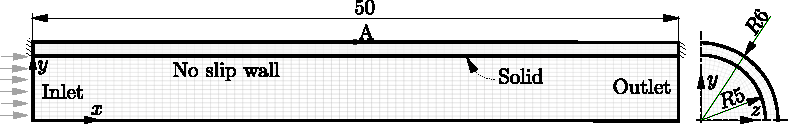
\includegraphics[scale=1]{figures/3dTube-geometry}
	\caption{Three-dimensional elastic tube: geometry and monitoring point A.}
	\label{fig:3dtube_geom}
\end{figure}

\paragraph{Purpose.}
A pressure pulse travelling through a fluid-filled elastic tube (Fig.~\ref{fig:3dtube_geom}) is the standard three-dimensional haemodynamic test of partitioned coupling under strong added mass ($\rho_s/\rho_f = 1.2$)~\citetodo{Formaggia et al.\ 2001; Gerbeau \& Vidrascu 2003; Fern\'andez \& Moubachir 2005}~\citep{kuttler2008fixed, Degroote2009}.
Most publications report only iteration counts and qualitative snapshots.

\paragraph{Problem.}
A quarter of the tube is modelled.
A $3\,\mathrm{ms}$ pressure pulse is applied at the inlet and the response is computed to $20\,\mathrm{ms}$, which includes the reflection from the outlet.
The fluid has $\rho_f = 1000\,\mathrm{kg/m^3}$, $\nu_f = 3\times10^{-6}\,\mathrm{m^2/s}$; the solid is Hookean linear elastic with small-strain kinematics (most published calculations use St Venant--Kirchhoff; the peak hoop strain is approximately $3\%$).

\paragraph{Reference.}
No tabulated values exist.
The available references are time histories at point A read from figures: \citet{Tukovic2018} (finite volume, BDF2, extracted exactly from vector graphics; same code lineage); and \citet{Lozovskiy2019} and \citet{Eken2016} (independent monolithic finite element codes, both using implicit Euler with $\Delta t = 10^{-4}\,\mathrm{s}$; raster-digitised to about $\pm3\times10^{-6}\,\mathrm{m}$).
The thick-wall long-wave estimate of the pulse-wave speed, $4.81\,\mathrm{m/s}$~\citep{Tukovic2018}, and the Moens--Korteweg speeds (5.2--5.7\,m/s) are approximate checks only.
The reference is therefore category C-weak.

\paragraph{Verification study.}
QoIs at point A are the maximum radial displacement $u_{r,\max}$ and its time, the incident trough of the axial displacement $u_{z,\min}$, the minimum radial displacement after reflection, the arrival time of the wavefront $t_\mathrm{arr}$ and the pulse-wave speed $c_p$.
The mesh study has two levels (16\,000 fluid/6\,400 solid cells and 128\,000/51\,200 cells, with $\Delta t$ halved); a third level (approximately $1.4\times10^6$ cells) is defined but has not been run.
The time-step study uses $\Delta t = 10^{-4}$ to $1.25\times10^{-5}\,\mathrm{s}$ on level 1.
A ``literature-discretisation'' run reproduces the implicit-Euler, $\Delta t = 10^{-4}\,\mathrm{s}$ set-up of the finite element references.
Robin--Neumann and IQN-ILS are compared on level 1.

\begin{table}[htbp]
	\centering
	\small
	\setlength{\tabcolsep}{5pt}
	\caption{3dTube: QoIs at point A on mesh levels 1 and 2 (BDF2, $\Delta t$ halved with the mesh), and the relative change between them.}
	\label{tab:3dtube}
	\begin{tabular}{lrrr}
		\toprule
		Quantity & Level 1 & Level 2 & Change \\
		\midrule
		$u_{r,\max}$ (mm) & 0.15984 & 0.15976 & $0.05\%$ \\
		$u_{z,\min}$ (mm) & $-0.08823$ & $-0.08660$ & $1.85\%$ \\
		$t_\mathrm{arr}$ (ms) & 5.874 & 5.854 & $0.34\%$ \\
		$c_p$ (m/s) & 4.771 & 4.695 & $1.58\%$ \\
		\bottomrule
	\end{tabular}
\end{table}

\paragraph{Findings.}
\begin{itemize}
	\item \emph{Time step.} Successive halvings of $\Delta t$ change $u_{r,\max}$ by $1.74\%$, $0.83\%$ and $0.016\%$, and $t_\mathrm{arr}$ by $2.23\%$, $0.44\%$ and $0.14\%$; the tutorial time step is converged to approximately $0.1\%$ in these QoIs.
	\item \emph{Mesh.} Between levels 1 and 2, $u_{r,\max}$ changes by only $0.05\%$, but $u_{z,\min}$ changes by $1.85\%$ and $c_p$ by $1.58\%$ (Table~\ref{tab:3dtube}). With two levels no order can be computed, and the axial displacement and wave speed are not yet shown to be converged.
	\item \emph{Literature discrepancy explained.} The published finite element peaks of $u_{r,\max}$ (approximately $0.119$ and $0.124\,\mathrm{mm}$) are some $21$--$24\%$ below the finite volume value of \citet{Tukovic2018} ($0.157\,\mathrm{mm}$). When the present code is run with the finite element discretisation in time (implicit Euler, $\Delta t = 10^{-4}\,\mathrm{s}$), its peaks lie within $+2.5\%$ of \citet{Lozovskiy2019} and $-1.4\%$ of \citet{Eken2016}. Most of the discrepancy between the finite element and finite volume literature is therefore explained by the numerical damping of the first-order, large-step time discretisation used in the published finite element calculations, not by the spatial discretisations or by the coupling.
	\item \emph{Converged comparison.} The level-2 BDF2 result, $u_{r,\max} = 0.15976\,\mathrm{mm}$, is $1.8\%$ above \citet{Tukovic2018}; $c_p = 4.695\,\mathrm{m/s}$ is $2.4\%$ below the approximate thick-wall estimate.
	\item \emph{Coupling.} Robin--Neumann and IQN-ILS histories differ by at most $0.27\%$ of the peak and the QoIs by at most $0.08\%$; Robin--Neumann needs 4.74 coupling iterations per step against 15.53 for IQN-ILS and is 4.1 times faster. The Robin--Neumann iteration count rises to 7.4 at the smallest time step; this has not been investigated.
\end{itemize}
% Derived: 0.1194/0.15694 - 1 = -23.9%; 0.1242/0.15694 - 1 = -20.9% (raster-digitised FE peaks vs Tukovic 2018 vector-extracted peak).

\todo{ESSENTIAL: run mesh level 3 (approximately $1.4\times10^6$ cells; estimated $>10$\,h on 6 ranks). Two levels do not support a convergence claim, and $u_{z,\min}$ still changes by $1.85\%$. COMSOL (or other independent code) solution with BDF2-type time integration at converged $\Delta t$ would add unique value: it would replace a same-lineage reference with an independent converged one and would test the time-discretisation explanation of the literature discrepancy from the finite element side.}

\paragraph{Role in the suite.}
This is the only three-dimensional transient case with mesh, time and coupling studies, and it yields a genuine ``benchmark revisited'' result: an apparent $\approx25\%$ disagreement between codes in the literature is largely a time-discretisation effect.
It also illustrates that a QoI-dependent conclusion is possible even with two mesh levels ($u_{r,\max}$ converged, $u_{z,\min}$ not).
Cost: level 1 425\,s and level 2 7\,197\,s on 4 ranks.
Limitations: two mesh levels; figure-digitised references; Hookean rather than St Venant--Kirchhoff solid; the pressure is ramped off over 3.0--3.1\,ms rather than instantaneously.

%%-------------------------------------------------------------------
\subsubsection{Modified lid-driven cavity}\label{sec:mok}
%%-------------------------------------------------------------------

\paragraph{Purpose.}
A lid-driven cavity with a flexible membrane bottom~\citetodo{Wall 1999 thesis; Mok 2001 thesis} is one of the oldest partitioned-coupling benchmarks~\citetodo{Gerbeau \& Vidrascu 2003}~\citep{kuttler2008fixed, Kassiotis2011}.
The membrane is tension-dominated (thickness $0.002\,\mathrm{m}$, $E = 250\,\mathrm{Pa}$) and undergoes large displacement (approximately $0.29\,\mathrm{m}$ in a $1\,\mathrm{m}$ cavity) under a periodically forced lid ($1-\cos(2\pi t/5)$); the cavity is nearly enclosed, with small openings that make the problem well posed for an incompressible fluid.

\paragraph{Reference: two inconsistent groups.}
The published midpoint histories fall into two mutually inconsistent groups (Fig.~\ref{fig:mok_refs}).
In group A (Mok, Wall, Gerbeau and Vidrascu) the openings are defined through the mesh and their size is not stated, so the problem depends on the mesh; the published peaks range from $0.177$ to $0.215\,\mathrm{m}$ and are not mutually consistent.
Group B (Vald\'es\citetodo{Vald\'es 2007 thesis}, the Kratos example\citetodo{Kratos Multiphysics example (Zorrilla)}, and Tiba et al.\citetodo{Tiba et al.\ 2026, arXiv:2609.16876 \emph{preprint}}) uses a fully specified inflow over a fixed $0.125\,\mathrm{m}$ opening and $p = 0$ at the outlet; within this group the peak displacement varies by $5.7\%$ and the oscillation amplitude by $20\%$.
\citet{Kassiotis2011} lies between the groups.
None of the published sources reports a mesh or time-step convergence study, and the Tiba et al.\ values are from a preprint and provide scalars only.
Two pilot runs show that the group-B definition reproduces group B, whereas traction-free conditions on both openings move the membrane downwards and reproduce neither group.
The reference is therefore category C-weak, and no single published value is treated as exact.

\begin{figure}[htbp]
	\centering
	% Source: solids4foam development, tutorials/fluidSolidInteraction/mokLidDrivenCavity/verification/reference/references_and_pilots.png (PR #497).
	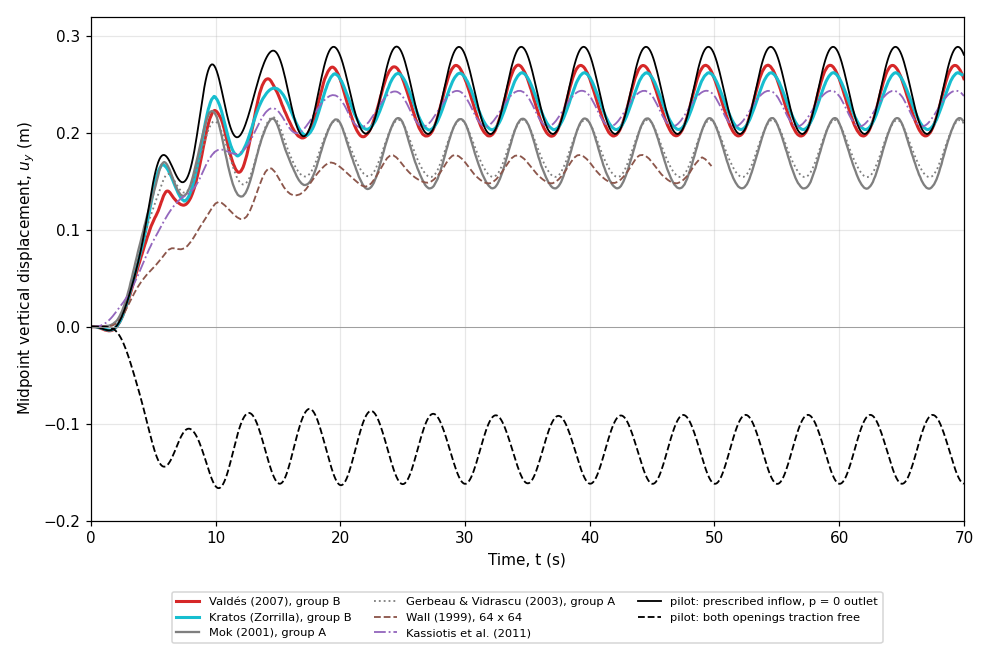
\includegraphics[width=0.85\textwidth]{figures/verification/mokLidDrivenCavity_references_and_pilots}
	\caption{Modified lid-driven cavity: published membrane-midpoint histories (group A: Mok, Wall, Gerbeau and Vidrascu; group B: Vald\'es, Kratos; Kassiotis et al.) and two pilot solids4foam runs ($32\times32$ mesh) with the group-B opening definition and with both openings traction free. Interim figure reproduced from the solids4foam verification output.}
	\label{fig:mok_refs}
\end{figure}
\todo{Replace Figure~\ref{fig:mok_refs} with a publication-quality figure that adds the converged ($96\times96$) solids4foam history and the group-B envelope, and drops the traction-free pilot or moves it to a separate panel. Confirm the extraction method and calibration of every curve before publication; the Kratos curve is raster-digitised (about $0.5\%$ of peak).}

\paragraph{Verification study.}
The QoIs are the mean peak, trough and time-mean of the membrane midpoint displacement over $t = 20$--$70\,\mathrm{s}$.
The mesh study uses $16^2$, $32^2$, $64^2$ and $96^2$ fluid cells with $\Delta t = 0.2$, $0.1$, $0.05$ and $0.025\,\mathrm{s}$; a $128^2$ run diverged (cause not isolated).
The time-step study uses $\Delta t = 0.1$, $0.05$ and $0.025\,\mathrm{s}$ on the $64^2$ mesh.
The standard solid (two or eight cells through the thickness) and the high-order solid are compared.

\begin{table}[htbp]
	\centering
	\small
	\setlength{\tabcolsep}{5pt}
	\caption{mokLidDrivenCavity: membrane-midpoint statistics (m) under combined mesh and time-step refinement, and the published group-B envelope. Group A peaks lie between 0.177 and 0.215\,m.}
	\label{tab:mok}
	\begin{tabular}{lrrr}
		\toprule
		Mesh ($\Delta t$) & Peak & Trough & Mean \\
		\midrule
		$16^2$ (0.2\,s) & 0.2934 & 0.1942 & 0.2426 \\
		$32^2$ (0.1\,s) & 0.2890 & 0.1986 & 0.2427 \\
		$64^2$ (0.05\,s) & 0.2870 & 0.2022 & 0.2437 \\
		$96^2$ (0.025\,s) & 0.2861 & 0.2044 & 0.2445 \\
		\midrule
		Group B envelope & 0.2619--0.2769 & 0.1967--0.2033 & 0.2316--0.2466 \\
		\bottomrule
	\end{tabular}
\end{table}

\paragraph{Findings.}
\begin{itemize}
	\item \emph{Self-convergence.} Successive changes in the peak are $1.56\%$, $1.26\%$ and $0.78\%$ of the peak; the observed order of the peak is approximately 1.2 (non-uniform final ratio), suggesting a limit near $0.285\,\mathrm{m}$, and that of the trough is below 0.5, leaving the trough uncertain by approximately $1$--$2\%$. The time step changes the response by $0.17\%$ and $0.04\%$ of the peak, so the error is dominated by the mesh.
	\item \emph{Comparison with the literature.} On the $96^2$ mesh the trough ($0.2044\,\mathrm{m}$) and the mean ($0.2445\,\mathrm{m}$) lie within or just outside the group-B envelope ($+0.56\%$ above the trough envelope), and the peak ($0.2861\,\mathrm{m}$) is $3.3\%$ above the largest group-B peak. Since the group-B sources are themselves single-mesh results that differ by $5.7\%$ in peak, this difference cannot be attributed to either side.
	\item \emph{Solid.} The standard and high-order solids agree to $0.04\%$: for a tension-dominated membrane the high-order solid gives no benefit (and costs 1.5 times more), in contrast to the bending-dominated collapsible channel (Section~\ref{sec:collapsible}).
	\item \emph{Coupling.} IQN-ILS needs 2.4--4.8 coupling iterations per step; Aitken relaxation needs approximately 9.9 and gives the same response (the difference has not been recorded quantitatively).
\end{itemize}

\paragraph{Role in the suite.}
The case is retained as an example of how a long-established benchmark can be ill defined: the literature contains two inconsistent problem definitions, neither supported by a convergence study.
The present results establish a self-converged solution for the fully specified group-B definition (to approximately $1\%$ in the peak, less well in the trough).
They are not a verification against an external reference.
\todo{An independent converged solution (COMSOL or another code) of the group-B definition, with its own mesh and time study, would add unique value and would make this a category-B case. Also: diagnose the $128^2$ divergence; Richardson estimates of peak and trough; quantify the IQN-ILS/Aitken difference.}


%%-------------------------------------------------------------------
\subsubsection{Flexible-bottom cavity [PROVISIONAL]}\label{sec:cavity}
%%-------------------------------------------------------------------

\todo{PROVISIONAL BENCHMARK: retain in main text only if (i) a clean partitioned mesh study with at least three levels in the asymptotic range is completed, including level 4 ($\Delta x = 0.0125$) at a reduced time step, together with a pseudo-time-step and coupling-tolerance check; and (ii) an independent converged reference (e.g.\ COMSOL, with its own mesh study) is obtained. The present reference is same-lineage and digitised (C-weak), and the steady displacement converges to a value approximately $5\%$ from it. All quasi-monolithic results for this case (simulationData/cavityFlexibleBottom, parent-paper Case~1) are deliberately NOT used as evidence. Otherwise move to supplementary material or drop.}

\begin{figure}[htbp]
	\centering
	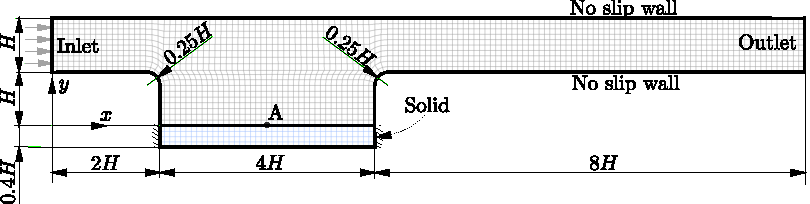
\includegraphics[scale=1]{figures/cavityFlexibleBottom-geometry}
	\caption{Channel flow over a cavity with a flexible bottom: geometry and boundary conditions.}
	\label{fig:cavity_geom_v}
\end{figure}

\paragraph{Why it could be valuable.}
Steady channel flow over a cavity with a flexible floor~\citep{Tukovic2018} (Fig.~\ref{fig:cavity_geom_v}), derived from a fluid benchmark~\citep{Juretic2010}, is the only steady internal-flow problem in the suite, and has large deformation of the floor ($u_y \approx -0.24\,\mathrm{m}$) at $Re = 100$.
It is inexpensive (about 10\,min serial for three levels).

\paragraph{Existing evidence.}
The reference is the mesh study of~\citet{Tukovic2018}, digitised from figures, computed with an earlier version of the same code family (category C-weak).
A partitioned (Aitken) mesh study with three levels ($\Delta x = 0.1$, $0.05$, $0.025\,\mathrm{m}$) gives steady displacements $u_y = -0.20246$, $-0.22883$ and $-0.23563\,\mathrm{m}$ at the monitoring point, i.e.\ $13.2\%$, $6.88\%$ and $5.59\%$ from the published values at the same spacing, with a net observed order of 1.96.
The interface force agrees with the published values to within $0.2\%$ on all three levels.
The displacement therefore converges at approximately second order, but towards a value about $5\%$ from the published curve, while the force agrees on every mesh.

\paragraph{Missing evidence.}
\begin{itemize}
	\item Level 4: diverges at the tutorial pseudo-time step ($\Delta t = 0.5\,\mathrm{s}$) with both Aitken and IQN-ILS, because the added-mass effect grows as interface cells shrink; it must be run with a smaller pseudo-time step.
	\item No coupling or tolerance study, and no partitioned pseudo-time-step study.
	\item The origin of the $5\%$ displacement offset at equal force is unexplained. Possible causes include a difference in solid model, material parameters, monitoring point or boundary conditions between the present set-up and that of~\citet{Tukovic2018}; an earlier solids4foam version gave $-0.219\,\mathrm{m}$ on the coarsest mesh, against $-0.20246\,\mathrm{m}$ now.
	\item An independent reference.
\end{itemize}

\paragraph{Promotion criterion.}
A clean partitioned three- to four-level study in the asymptotic range, an explanation of the displacement offset, and an independent converged COMSOL solution of the identical set-up.
If the independent solution agrees with the present converged displacement, the case would demonstrate that a same-lineage published curve was inaccurate; if it agrees with the published curve, it would expose a set-up or modelling difference.
Either outcome is informative, but neither can be claimed now.


%%%%%%%%%%%%%%%%%%%%%%%%%%%%%%%%%%%%%%%%%%%%%%%%%%%%%%%%%%%%%%%%%%
\subsection{Three-dimensional and realistic-complexity benchmarks}\label{sec:threeD}
%%%%%%%%%%%%%%%%%%%%%%%%%%%%%%%%%%%%%%%%%%%%%%%%%%%%%%%%%%%%%%%%%%

%%-------------------------------------------------------------------
\subsubsection{Beam in cross-flow [PROVISIONAL]}\label{sec:beam}
%%-------------------------------------------------------------------

\todo{PROVISIONAL BENCHMARK: retain in main text only if (i) a graded fluid-mesh family that resolves the near-body flow and boundary layer reaches the asymptotic range for both displacement and integrated force (three levels with consistent observed orders), with per-level values tabulated in CSV; and (ii) an independent converged reference is obtained, at least for the large-deformation (modified) form (COMSOL; or Gillebaart et al.\ 2016 if it tabulates the same configuration). Current uniform refinements are NOT asymptotic, and no convergence claim may be made from them.}

\begin{figure}[htbp]
	\centering
	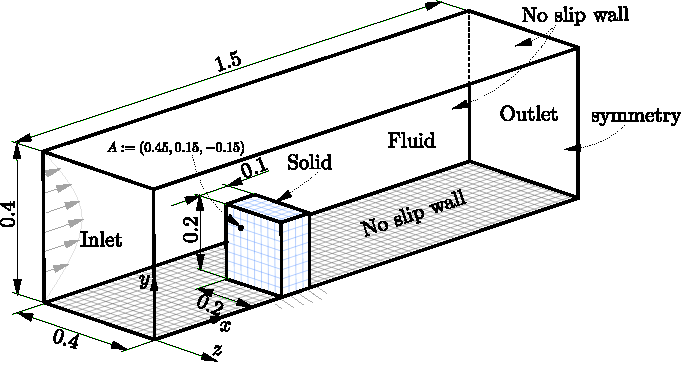
\includegraphics[scale=1]{figures/beamInCrossFlow-geometry}
	\caption{Beam in cross-flow: geometry (half domain with $z = 0$ symmetry) and monitoring point A.}
	\label{fig:beam_geom}
\end{figure}

\paragraph{Why it could be valuable.}
A thick elastic plate clamped in a three-dimensional channel flow (Fig.~\ref{fig:beam_geom}) is the only steady three-dimensional case in the suite, and the only three-dimensional large-deformation case.
Two forms share one geometry: an original small-deformation form ($E = 1.4\,\mathrm{MPa}$, $U_\mathrm{max} = 0.2\,\mathrm{m/s}$, $Re = 40$)~\citep{Richter2015} and a modified large-deformation form ($E = 10\,\mathrm{kPa}$, $U_\mathrm{max} = 0.3\,\mathrm{m/s}$)~\citep{Tukovic2018}, which together separate geometric nonlinearity from discretisation effects.

\paragraph{Existing evidence.}
\begin{itemize}
	\item \emph{References.} Original form: $u_x(A) = 5.95\times10^{-5}\,\mathrm{m}$ and $F_x = 1.33\,\mathrm{N}$ from an independent monolithic finite element code~\citep{Richter2015} (category C; which refinement level, and whether the values are extrapolated, remains to be checked). Modified form: values read from Fig.~28 of \citet{Tukovic2018}, a single unstructured mesh computed with an earlier version of the same code family (category C-weak).
	\item \emph{Mesh studies.} Uniform refinements by factors 1, 2, 4, 8 (original; finest approximately $7.6\times10^6$ cells, about 11\,h on 64 cores) and 1, 2, 3, 4, 8 (modified), with $\Delta t$ reduced with the mesh. On the finest original mesh, $u_x(A) = 5.95387\times10^{-5}\,\mathrm{m}$ ($+0.07\%$ from Richter) and $F_x = 1.310774\,\mathrm{N}$ ($-1.4\%$ from Richter). On the finest modified mesh the displacements differ from the same-lineage values by $-2.3\%$ ($u_x$), $-0.7\%$ ($u_y$) and $+2.3\%$ ($2u_z$).
	\item \emph{Non-asymptotic behaviour.} The final refinement still changes $u_x(A)$ by approximately $4.6\%$ (original) and $4.7\%$ (modified) (values read from the stored plots), and the transverse force $F_y$ (original) varies non-monotonically. The close agreement of the finest $u_x(A)$ with Richter therefore cannot be separated from coincidence.
	\item \emph{Displacement versus force.} On the finest original mesh $u_x(A)$ agrees with Richter to $0.07\%$ while $F_x$ differs by $1.4\%$, and the two converge differently under refinement. This is consistent with the integrated force being controlled by the resolution of the near-body velocity gradients, which uniform refinement of a coarse base mesh improves only slowly; it is a hypothesis to be tested by the graded-mesh study, not an established result.
	\item \emph{Coupling.} Robin--Neumann and IQN-ILS agree to within $0.4\%$ on the base mesh for both forms. The refined meshes were not re-run after a later change of the IQN-ILS default settings, which changed the base-mesh result by $0.01\%$.
\end{itemize}

\paragraph{Missing evidence and promotion criterion.}
\begin{itemize}
	\item A graded fluid-mesh family with boundary-layer resolution near the plate, reaching consistent three-level observed orders for $u_x(A)$, $u_y(A)$, $F_x$ and $F_y$, with Richardson estimates.
	\item Tabulated per-level values (currently only the finest values are tabulated; the others are read from plots).
	\item An independent time-step check (none exists; $\Delta t$ is scaled with the mesh).
	\item Confirmation of the Richter refinement level; an independent converged reference for the modified form (COMSOL, or Gillebaart et al.~\citep{Gillebaart2016} if applicable).
\end{itemize}

%%-------------------------------------------------------------------
\subsubsection{Hessenthaler three-dimensional benchmark [IN DEVELOPMENT]}\label{sec:hessenthaler}
%%-------------------------------------------------------------------

\todo{IN DEVELOPMENT --- placeholder only. No solids4foam case, verification driver or numerical result for this benchmark exists in the repository at the time of writing. Do not add numbers until the case and its verification study exist. Retain in the main text only if mesh, time-step and coupling-tolerance studies are completed with consistent observed orders for the principal QoIs.}

\paragraph{Intended role.}
The benchmark of Hessenthaler et al.\citetodo{Hessenthaler et al.\ 2017, IJNMBE, ``Experiment for validation of fluid--structure interaction models and algorithms''; check also the companion numerical paper} is intended as the realistic-complexity, fully three-dimensional capstone of the suite: a geometrically complex, three-dimensional, large-deformation FSI problem driven by periodic flow, at a cost that tests solver robustness and parallel performance rather than a single coupling mechanism.

\paragraph{Planned verification study.}
\begin{itemize}
	\item Problem definition and parameters taken from the published specification; deviations stated explicitly.
	\item QoIs to be defined (e.g.\ membrane/structure displacement at defined points, flow rate, pressure drop), with periodic-window statistics as in Section~\ref{sec:qoi}.
	\item Mesh study (at least three levels), time-step study (at least three levels) and a coupling-tolerance sweep, each with observed orders.
	\item An independent numerical reference, if available (COMSOL or published), classified according to Table~\ref{tab:ref_hierarchy}.
\end{itemize}

\paragraph{Experimental data.}
The benchmark is accompanied by phase-contrast MRI and other experimental measurements.
These are \emph{validation} data: agreement with them depends on the mathematical model as well as on the numerics, and they are not used as evidence of numerical verification in this paper.
If included, they will be presented separately, as context, after the numerical verification.


%%%%%%%%%%%%%%%%%%%%%%%%%%%%%%%%%%%%%%%%%%%%%%%%%%%%%%%%%%%%%%%%%%
\subsection{Additional transient benchmark}\label{sec:additional}
%%%%%%%%%%%%%%%%%%%%%%%%%%%%%%%%%%%%%%%%%%%%%%%%%%%%%%%%%%%%%%%%%%

%%-------------------------------------------------------------------
\subsubsection{Blob in treacle [PROVISIONAL]}\label{sec:blob}
%%-------------------------------------------------------------------

\todo{PROVISIONAL BENCHMARK / possible supplementary material: retain in the main text only if (i) an independent converged reference (COMSOL being arranged) replaces the coarse, figure-digitised preprint reference; and (ii) the time study is extended below $\Delta t = 0.03125\,\mathrm{s}$ with tightened coupling and solver tolerances, showing orders close to 2 rather than the present super-nominal 2.4--2.5. Otherwise move to supplementary material.}

\begin{figure}[htbp]
	\centering
	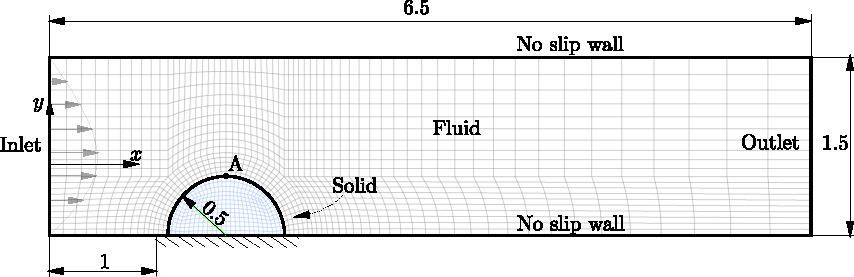
\includegraphics[scale=1]{figures/blobInTreacle-geometry}
	\caption{Blob in treacle: elastic half-cylinder in a viscous channel flow; geometry and monitoring (top) point.}
	\label{fig:blob_geom}
\end{figure}

\paragraph{Why it could be valuable.}
An elastic half-cylinder in a highly viscous channel flow (Fig.~\ref{fig:blob_geom}; $\rho_f = 1$, $\nu_f = 1$, ramped to a steady state at $t = 2\,\mathrm{s}$), proposed by~\citet{Liu2014} to measure the temporal order of a coupled scheme, is a strongly damped, large-deformation problem (top-point $u_x \approx 0.12\,\mathrm{m}$ for a $0.1\,\mathrm{m}$ radius) in which the temporal error can be isolated cleanly.

\paragraph{Existing evidence.}
\begin{itemize}
	\item \emph{Reference (C-weak).} \citet{Liu2014} report only self-convergence norms. The preprint version\citetodo{Liu et al., arXiv:1401.0082} gives interface shapes at $t = 1\,\mathrm{s}$ (P5/P4/P5 elements, first-order time integration with $\Delta t = 0.025\,\mathrm{s}$, with an estimated time error of approximately $4\%$ of its own) and at steady state (a coarse mesh of 1\,239 fluid and 370 solid triangles); these were vector-extracted from figures.
	\item \emph{Time step.} At $t = 1\,\mathrm{s}$, $\Delta t = 0.25$, $0.125$, $0.0625$, $0.03125\,\mathrm{s}$ give top-point $u_x = 0.0558737$, $0.0564184$, $0.0565219$ and $0.0565398\,\mathrm{m}$, with observed orders 2.39 and 2.54 ($u_x$) and 2.39 and 2.41 (interface shape). Below $\Delta t = 0.03125\,\mathrm{s}$ the changes reach the coupling/solver-tolerance level (approximately $10^{-5}\,\mathrm{m}$). Orders above the formal value of 2 indicate that this large-$\Delta t$ sequence is not yet in the asymptotic range; the evidence supports ``at least second-order'' behaviour over this range, not a measured order of 2.
	\item \emph{Mesh.} Four levels (factors 0.5--4) give steady $u_x = 0.108206$, $0.117301$, $0.119698$, $0.120152\,\mathrm{m}$, with an observed order of 2.40 and a Richardson estimate of $0.12026\,\mathrm{m}$; the finest level is within $0.1\%$ of it.
	\item \emph{Comparison.} At $t = 1\,\mathrm{s}$ the interface shape is within $1.6\%$ of the preprint, inside its own approximately $4\%$ time error. At steady state, $u_x$ is $7.4\%$ smaller than the preprint value and $|u_y|$ $20\%$ larger; this offset is attributed to the coarseness of the reference mesh, but this attribution is unconfirmed.
	\item \emph{Coupling.} No coupling comparison or tolerance study exists; the finest mesh requires $\Delta t = 0.005\,\mathrm{s}$ because of IQN-ILS stagnation.
\end{itemize}

\paragraph{Promotion criterion.}
An independent converged reference at $t = 1\,\mathrm{s}$ and at steady state; a time study extended to smaller $\Delta t$ with tightened tolerances; a coupling-tolerance check.
The case's distinctive contribution, a clean temporal-order measurement in a viscous large-deformation problem, partly overlaps with ringAddedMass and collapsibleChannel, which is why it may ultimately be moved to supplementary material.
